%%%%%%%%%%%%%%%%%%%%%%%%%%%%%%%%%%%%%%%%%%%%%%%%%%%%%%%%%%%%%%%%%%%%%%
% CS671: Machine Learning
% Copyright 2015 Pejman Ghorbanzade <mail@ghorbanzade.com>
% Creative Commons Attribution-ShareAlike 4.0 International License
% More info: https://bitbucket.org/ghorbanzade/umb-cs671-2015s
%%%%%%%%%%%%%%%%%%%%%%%%%%%%%%%%%%%%%%%%%%%%%%%%%%%%%%%%%%%%%%%%%%%%%%

\section*{Question 1}

A rhombus $R_{x_0, y_0, c, d}$ is a quadrilateral which has the vertices $(x_0-c, y_0)$, $(x_0, y_0-d)$, $(x_0+c, y_0)$, $(x_0, y_0+d)$ as shown in Figure \ref{fig11}.
Prove that the class of rhombi  in $\mathbb{R}^2$ for which the ratio $c/d$ is a constant is a PAC-learnable.

\begin{figure}[H]
\centering
\begin{tikzpicture}
\begin{axis}[axis lines = middle, axis equal, ticks = none, xmin = -.5, xmax = 5.5, ymin = 1, ymax = 3, xlabel = {$x$}, ylabel = {$y$}, clip=false]
\addplot[domain=1:4]{(7-x)/3};
\addplot[domain=4:7]{(x-1)/3};
\addplot[domain=1:4]{(x+5)/3};
\addplot[domain=4:7]{(13-x)/3};
\addplot[loosely dashed] coordinates {(4,0.5) (4,3.5)};
\addplot[loosely dashed] coordinates {(0.5,2) (7.5,2)};
\addplot[mark=*] coordinates {(1,2)} node[above left] {$(x_0-c,y_0)$};
\addplot[mark=*] coordinates {(4,1)} node[below left] {$(x_0, y_0-d)$};
\addplot[mark=*] coordinates {(4,3)} node[above right] {$(x_0, y_0+d)$};
\addplot[mark=*] coordinates {(7,2)} node[below right] {$(x_0+c, y_0)$};
\end{axis}
\end{tikzpicture}
\caption{Rhombus having vertices $(x_0-c, y_0)$, $(x_0, y_0-d)$, $(x_0+c, y_0)$, $(x_0, y_0+d)$}\label{fig11}
\end{figure}

\subsection*{Solution}

Set of possible examples $\mathcal{X}$ is $\mathbb{R}^2$.
$\mathcal{R}$ is set of all rhombi with ratio $c/d$.
Therefore, the concept $\mathcal{C}$ would be a particular rhombus with ratio $c/d$.

Suppose the rhombus shown in Figure \ref{fig11} is a concept $c \in \mathcal{C}$ which is not known by the learner.

As the hypothesis $h_S$, formed by the learner, is also a rhombus, Figure \ref{fig12} can be constructed in which $h_S$ is the rhombus formed by intersection of dashed lines.
Areas enclosed by dashed lines and different edges of the concept rhombus are defined as $r_1$, $r_2$, $r_3$ and $r_4$.

\begin{figure}[H]
\centering
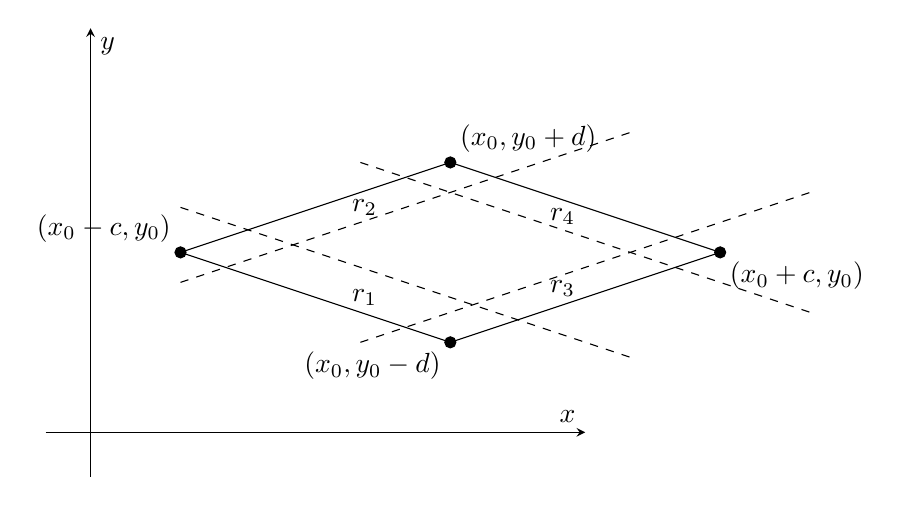
\begin{tikzpicture}
\begin{axis}[axis lines = middle, axis equal, ticks = none, xmin = -.5, xmax = 5.5, ymin = 1, ymax = 3, xlabel = {$x$}, ylabel = {$y$}, clip=false]

\addplot[domain=1:4]{(7-x)/3};
\addplot[domain=4:7]{(x-1)/3};
\addplot[domain=1:4]{(x+5)/3};
\addplot[domain=4:7]{(13-x)/3};

\addplot[mark=*] coordinates {(1,2)} node[above left] {$(x_0-c,y_0)$};
\addplot[mark=*] coordinates {(4,1)} node[below left] {$(x_0, y_0-d)$};
\addplot[mark=*] coordinates {(4,3)} node[above right] {$(x_0, y_0+d)$};
\addplot[mark=*] coordinates {(7,2)} node[below right] {$(x_0+c, y_0)$};

\addplot[domain=1:6, dashed]{(8.5-x)/3};
\addplot[domain=3:8, dashed]{(12-x)/3};
\addplot[domain=3:8, dashed]{(x)/3};
\addplot[domain=1:6, dashed]{(x+4)/3};

\addplot[mark=none] coordinates {(2.8,1.7)} node[below right] {$r_1$};
\addplot[mark=none] coordinates {(2.8,2.7)} node[below right] {$r_2$};
\addplot[mark=none] coordinates {(5,1.8)} node[below right] {$r_3$};
\addplot[mark=none] coordinates {(5,2.6)} node[below right] {$r_4$};

\end{axis}
\end{tikzpicture}
\caption{Rhombus having vertices $(x_0-c, y_0)$, $(x_0, y_0-d)$, $(x_0+c, y_0)$, $(x_0, y_0+d)$}\label{fig12}
\end{figure}

Suppose the probability of the generalization error defined as in Equation \ref{eq11} would be less than $\epsilon$.

\begin{equation}\label{eq11}
R(h) = P({x\in \mathcal{X} | h_s(x) \neq c(x)})
\end{equation}

This means that probability of the hypothesis $h_S$ is at least $1 - \epsilon$.
This means that the rhombus $h_s$ must intersect at least one of $r_1$, $r_2$, $r_3$ or $r_4$.
Therefore,

\begin{equation}
\begin{aligned}
P(R(h_S)>\epsilon) &\leq P_{S~D}( \bigcup_{i=1}^{4}[(h_S \cap r_i)] = \emptyset )\\
&\leq \sigma_{i=1}^{4} P((h_S \cap r_i) = \emptyset)\\
&\leq 4(1 - \frac{\epsilon}{4})^m
\end{aligned}
\end{equation}

Since for all $x \in \mathbb{R}$ we have $1 - x \leq \exp^{-x}$,

\begin{equation}
\begin{aligned}
P(R(h_S)>\epsilon) &\leq 4(1 - \frac{\epsilon}{4})^m\\
&\leq 4 \times \exp^{-\frac{m\epsilon}{4}}
\end{aligned}\label{eq13}
\end{equation}

Since $P(R(h_S) > \epsilon) \leq \delta$,

\begin{equation}\label{eq14}
4\exp^{-\frac{m\epsilon}{4}} \leq \delta
\end{equation}

Therefore,

\begin{equation}\label{eq15}
m \geq \frac{4}{\epsilon} \log \frac{4}{\delta}
\end{equation}

Given that $\log u \leq u - 1$,

\begin{equation}\label{eq16}
\begin{aligned}
m &\geq \frac{4}{\epsilon} \log \frac{4}{\delta}\\
& \geq \frac{4}{\epsilon} (\frac{4}{\delta} - 1)
\end{aligned}
\end{equation}

And we have shown that there is a polynomial $p(\frac{1}{\epsilon}, \frac{1}{\delta})$ such that if $m \geq p(\frac{1}{\epsilon},\frac{1}{\delta},n,size(c))$, then there is an algorithm producing $h_S$ such that $P(R(h_s) \leq \epsilon) \geq 1 - \delta$.
Hence we have shown by definition that the class of rhombi with ratio $c/d$ is PAC learnable.
